\pgfplotsset{
	axis lines=middle,
	axis line style={->},
	xmin=0,
	xticklabels=empty,
	xtick=\empty,
	ymin=-1.2,
	ymax=1.2,
	yticklabels=empty,
	ytick=\empty,
	samples=200,
	every axis plot post/.append style={very thick},
	clip=true,
}% end of common axis set
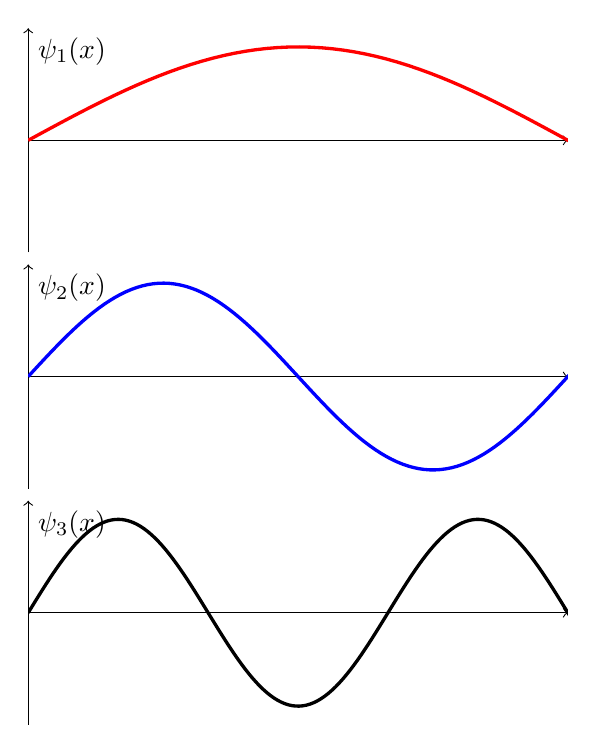
\begin{tikzpicture}
	\begin{axis}% 1. plot
		[
		domain=0:4*pi,
		xmax=pi,
		yscale=0.5,
        ylabel={$\psi_1(x)$},
		]
		\addplot[red] {sin(deg(x+pi))*-1};
	\end{axis}
	\begin{axis}% 2. plot
		[
		domain=0:4*pi,
		xmax=2*pi,
		yshift=-3cm,
		yscale=0.5,
        ylabel={$\psi_2(x)$},
		]
		\addplot[blue] {sin(deg(x+pi))*-1};
	\end{axis}
	\begin{axis}% 3. plot
		[
		domain=0:4*pi,
		xmax=3*pi,
		yshift=-6cm,
		yscale=0.5,
        ylabel={$\psi_3(x)$},
		]
		\addplot[black] {sin(deg(x+pi))*-1};
	\end{axis}
\end{tikzpicture}
